\documentclass{paper}

%\usepackage{times}
\usepackage{epsfig}
\usepackage{graphicx}
\usepackage{amsmath}
\usepackage{amssymb}
\usepackage{color}
\usepackage{mathtools}




\usepackage{caption}
\usepackage{float}
\usepackage{subfigure}


% load package with ``framed'' and ``numbered'' option.
%\usepackage[framed,numbered,autolinebreaks,useliterate]{mcode}

% something NOT relevant to the usage of the package.
\setlength{\parindent}{0pt}
\setlength{\parskip}{18pt}





\newcommand{\prox}{\text{prox}}

\newcommand{\twonorm}[1]{\left\lVert#1\right\rVert_2}
\usepackage[latin1]{inputenc} 
\usepackage[T1]{fontenc} 


\usepackage[latin1]{inputenc} 
\usepackage[T1]{fontenc} 

\usepackage{listings} 
\lstset{% 
   language=Matlab, 
   basicstyle=\small\ttfamily, 
} 

\newcommand{\norm}[1]{\left\lVert#1\right\rVert}
\DeclareMathOperator*{\argmin}{arg\,min}

\title{Project 2 - Demosaicing}



\author{Single Michael\\08-917-445}
% //////////////////////////////////////////////////


\begin{document}



\maketitle


\section{Problem Statement}

In this work we address the problem of demosaicing by formulating it as a convex optimization problem. Given a mosaiced image $g$ depicting a raw camera production, we want to find an optimal demosaiced image $u$. For describing the optimality property we take into account a cost function that describes the color smoothness and also that the resulting image $u$ should be close to the given raw input image $g$. 

More precisely, let $g$ denote the bayer filter camera raw input image. Then we want to solve for $u=(u_r, u_g, u_g)$ (RGB image) minimzating the following energy term (cost function):

\begin{align}
	E(u_c) = \norm{\nabla u_c}_2 + \frac{\lambda}{2} \norm{u_c - g}^2_{\Omega_{c}}
\label{eq:basis_cost_demosaicing}	
\end{align}

with the measure

\begin{equation}
	\norm{u_C - g}^2_{\Omega_{C}} = \sum_x \sum_y \Omega_{C}(x,y)\norm{u_{c}(x,y) - g(x,y)}^2
\label{eq:measure}
\end{equation}


where C denotes the three different color channels. $\Omega_{C}$ is defined such that $\Omega_{C}(x,y) = 1$ if the pixel value at $(x,y)$ is \emph{valid}$\footnote{this means that the pixel at location (x,y) is valid for the bayer color mask C}$ and $\Omega_{C}(x,y) = 0$ when the data is missing.

The cost function from equation $\ref{eq:basis_cost_demosaicing}$ consists of a smoothness term, $\norm{\nabla u_c}_2$ and $\norm{u_c - g}^{2}_{\Omega_{c}}$. The first term ensures a smooth color transition between colors in a l2 norm sense. The second term ensures that the reconstructed images does not deviate too much from the given input, i.e. de demosaiced image should resemble to the provided mosaiced raw camera image. This similarity term is further parameterized by a regularization term $\lambda$, indicating how strong the output should match the given input according to the formulated measure in equation $\ref{eq:measure}$. In summary, larger values for $\lambda$ weight the similarity of the input and output image more, and contrarely, lower values weight the color smoothness term more.

Hereby, minimizating the cost function from equation $\ref{eq:basis_cost_demosaicing}$ leads to an optimal demosaiced image $u$.
Mathematically we want to solve for 

\begin{equation}
	\widetilde{u} = \argmin_{u_c} E(u_c)
\label{eq:our_general_cost_function}
\end{equation}

We can further simplify the cost function stated in equation $\ref{eq:basis_cost_demosaicing}$ relying on the following observation: Since the function $\Omega_{C}$ is only true for pixels that correspond to the color channel C in the bayer mask, we see that $\Omega_{C}(x,y)\norm{u_{c}(x,y) - g(x,y)}$ is only not equal zero if the pixel at location $(x,y)$ belongs to the color channel $C$. Therefore we are allowed to solve the stated optimization problem from equation $\ref{eq:basis_cost_demosaicing}$ for each color channel separately. 


According to this insight we are supposed to minimize the following three independent$\footnote{Independent in the sense that we are allowed to solve for each color channel separately}$ convex problems:



\begin{align}
	\widetilde{u}_R = \argmin_{u_R} \norm{\nabla u_R}_2 + \frac{\lambda}{2} \norm{u_R - g}^2_{\Omega_{R}} \nonumber \\
	\widetilde{u}_G = \argmin_{u_G} \norm{\nabla u_G}_2 + \frac{\lambda}{2} \norm{u_G - g}^2_{\Omega_{G}}\nonumber \\
	\widetilde{u}_B = \argmin_{u_B} \norm{\nabla u_R}_2 + \frac{\lambda}{2} \norm{u_B - g}^2_{\Omega_{B}}
\label{eq:our_convex_probelm}		
\end{align}

Where we still rely on the measure defined in equation $\ref{eq:measure}$ but C was replayed by the appropriate color channel$\footnote{C stands for either the color channel R, G or B.}$. We notice that the equations in $\ref{eq:our_convex_probelm}$ tell us that we have to solve three different energies similar to the one formulated in equation $\ref{eq:our_general_cost_function}$.

In the next section we will describe how to solve the stated minimization problems from equation $\ref{eq:our_convex_probelm}$ numerically.


\section{Primal-Dual Form}
In this section we derive the primal-dual form of the stated convex demosaicing problem.

But first off, let us consider an initial problem of the form 

\begin{align}
	\min_{x \in X} F(K x) + G(x)
\label{eq:initial_primal}	
\end{align}

where $F$, $G$ are convex functions and $K$ denotes a linear operator. 

The primal-dual formulation for equation $\ref{eq:initial_primal}$ is given by 

\begin{align}
	\min_{x \in X} \max_{y \in Y} < Kx, y > - F^*(y) + G(x)
\label{eq:initial_primal_dual}	
\end{align}


For a given mosaiced RGB image $u_{RGB}$ encoded as a 3 dimensional $M \times N$ matrix, i.e. a tensor of dimension $M \times N \times 3$. As mentioned in the problem statement we can solve three independent convex problems in order to solve the problem of demosaicing a RGB image. Therefore let in the following $u$ define stand for one particular color channel of the given color image $u_{RGB}$.

\begin{equation}
\min_{u \in U} \norm{\nabla u} + \frac{\lambda}{2} \norm{u - g}^2_{\Omega}
\label{eq:initial_energy}
\end{equation}

where $\norm{u - g}^2_{\Omega}$ is defined as in equation $\ref{eq:measure}$ and $g$ is the corresponding color channel of the mosaiced image described in the problem statement.

We observe that equation $\ref{eq:initial_energy}$ has the same structure as the initial problem stated in equation $\ref{eq:initial_primal}$. This allows us to formulate the primal-dual form of equation $\ref{eq:initial_energy}$ which will look like the following:

\begin{align}
	\min_{u \in U} \max_{y \in Y} < Kx, y > - F^*(y) + G(x)
\label{eq:initial_primal_dual}	
\end{align}

Where $K$, $F$ and $G$ are defined as:

\begin{align}
	K &= \nabla \nonumber \\
	F &= \norm{\cdot}_2 \nonumber \\
	G &= \norm{u - g}^2_{\Omega}
\label{eq:def_kfg}	
\end{align}

Note that $F*$ denotes the convex conjugate form of $F$. The convex conjugate of $F$ has an explicit identity that can be computed using the Legendre-Fenchel-Transform.

\begin{align}
	F^*(y) &= (\norm{\cdot}_2)^*(y) \nonumber \\
		  &= \sup_x x^T y - \twonorm{x} \nonumber \\
		  &= \sup_x x^T y - \max_{\twonorm{z} \leq 1} x^T z \nonumber \\
		  &= \sup_x \min_{\twonorm{z} \leq 1} x^T(y-z) \nonumber \\
		  &= \begin{cases}
   				0  			& \text{if} \twonorm{y} \leq 1 \\
   				\infty      & \text{otherwise}
  			 \end{cases} \nonumber \\
  		  &= \delta(y)
\label{eq:legendre_fenchel_transform_f}  		  
\end{align}

The first equality is simply the definition of $F$. The second equality is using the so called Legendre-Fenchel transformation,

\begin{equation}
	(\norm{\cdot}_2)^*(y) = \sup_x x^T y - \twonorm{x} \nonumber
\end{equation}. 

In the third equality I make use of the Cauchy-Schwarz inequality, 
\begin{equation}
	\twonorm{x} = \max_{\twonorm{z} \leq 1} x^T z
\end{equation}


Plugging equation $\ref{eq:legendre_fenchel_transform_f}$ and the definitions in from equation $\ref{eq:def_kfg}$ into the primal-dual equation equation $\ref{eq:initial_primal_dual}$ we conclude the following final primal-dual formulation:

\begin{equation}
\min_{u \in U} \max_{y \in Y} <\nabla u, y> - \delta(y) + \frac{\lambda}{2}\norm{u - g}^2_{\Omega}
\label{eq:final_primal_dual}
\end{equation}


\section{Primal-Dual steps}
In this section I will present an iterative solver for our stated primal-dual formulation.

In the following I am going to rely on an algorithm formulated by A.Chambolle and T.Pocke which allows to solve primal-formulations as ours stated in equation $\ref{eq:final_primal_dual}$.
They stated an iterative algorithm that has the following update steps:

\begin{align}
	y^{n+1} &= \prox_{\sigma F^*}(y^n + \sigma K \bar{x}^n) \nonumber \\
	x^{n+1} &= \prox_{\tau G}(x^n - \tau K^* y^{n+1}) \\
	\bar{x}^{n+1} &= x^{n+1} + \theta(x^{n+1} - x^n)
\label{eq:update_rules_plain}	
\end{align}
with $\theta \in (0, 1]$ and the constraint $\tau \sigma \norm{K}^2 < 1$. Note that stated constraint is important in order to guarantee convergence of their algorithm.

Hereby $prox(\cdot)$ denotes the proximity operator and is defined as 

\begin{equation}
	\prox_{\lambda F}(z) = \arg \min_x \frac{1}{2} \twonorm{x - z}^2 + \lambda F(x)
\end{equation}

In the following we will derive explicit identities for the update rules in equation $\ref{eq:update_rules_plain}$that can be numerically solved. Our goal is to find an expression for the proximity operator.

\subsection{Update for $y^{n+1}$}

In this subsection we derive an identity for the $y^{n+1}$ update rule from equation $\ref{eq:update_rules_plain}$. The key idea is to use the so called Moreau's Identity:  

\begin{equation}
	\prox_{\lambda F^*}(z) = z - \lambda \cdot \prox_{F/ \lambda}(z / \lambda) 
\label{eq:moreau}	
\end{equation}

Next, we apply the Moreau's identity to the proximity operator of the Legendre-Fenchel transformation.


\begin{align}
	\prox_{\lambda F^*}(y^n + \sigma K \bar{x}^{n}) 
	&= (y^n + \sigma K \bar{x}^{n}) - \sigma \prox_{\frac{F}{\sigma} } \left(\frac{y^n + \sigma K \bar{x}^{n} }{\sigma} \right) \nonumber \\
	&= (y^n + \sigma K \bar{x}^{n}) - \sigma \left( \frac{y^n + \sigma K \bar{x}^{n} }{\sigma} \max{0, 1-\frac{1}{\twonorm{y^n + \sigma K \bar{x}^{n} }}} \right) \nonumber \\
	&= (y^n + \sigma K \bar{x}^{n}) - \left( y^n + \sigma K \bar{x}^{n} \right) \max{\left(0, 1-\frac{1}{\twonorm{y^n + \sigma K \bar{x}^{n} }}\right)}  
\label{eq:y_n_1_expression}
\end{align}

For the first equality we use the definition of equation $\ref{eq:moreau}$ and for the second equality we used the fact (proven during class) that

\begin{align}
	\prox_{\frac{\twonorm{\cdot}}{\sigma}}(\frac{x}{\sigma}) = \frac{x}{\sigma} \max{\left(0, 1-\frac{1}{\twonorm{x}}\right)}
\end{align}

To simplify our derivation even and also get rid of the proximity operator we next make a case distinction for $\twonorm{y^n + \sigma K \bar{x}^{n}}$. 

\begin{itemize}
	\item If $\twonorm{y^n + \sigma K \bar{x}^{n}} \geq 1$
		then  
		\begin{align}
			0 \leq 1-\frac{1}{\twonorm{y^n + \sigma K \bar{x}^{n}}} \leq 1
		\end{align}
		
		Therefore $\frac{1}{\twonorm{y^n + \sigma K \bar{x}^{n}}}$ is smaller than one and thus
		
		\begin{align}
			\max{\left(0, 1-\frac{1}{\twonorm{y^n + \sigma K \bar{x}^{n}}}\right)} 
			&= 1-\frac{1}{\twonorm{y^n + \sigma K \bar{x}^{n}}}
		\end{align}
		
		This insight can directly be used for the maximum expression in equation $\ref{eq:y_n_1_expression}$ and we hence obtain:
		
		\begin{align}
			\prox_{\lambda F^*}(y^n + \sigma K \bar{x}^{n})
			&= (y^n + \sigma K \bar{x}^{n}) - \left( y^n + \sigma K \bar{x}^{n} \right) \max{\left(0, 1-\frac{1}{\twonorm{y^n + \sigma K \bar{x}^{n} }}\right)} \nonumber \\
			&= (y^n + \sigma K \bar{x}^{n}) - \left( y^n + \sigma K \bar{x}^{n} \right) \left( 1-\frac{1}{\twonorm{y^n + \sigma K \bar{x}^{n}}} \right)\nonumber \\
			&= (y^n + \sigma K \bar{x}^{n}) -(y^n + \sigma K \bar{x}^{n}) +\frac{y^n + \sigma K \bar{x}^{n}}{\twonorm{y^n + \sigma K \bar{x}^{n}}} \nonumber \\
			&= \frac{y^n + \sigma K \bar{x}^{n}}{\twonorm{y^n + \sigma K \bar{x}^{n}}}
		\end{align}
		
	\item If $\twonorm{y^n + \sigma K \bar{x}^{n}} < 1$
		then 
		\begin{align}
			1-\frac{1}{\twonorm{y^n + \sigma K \bar{x}^{n}}} < 0
		\end{align}
		thus we conclude 
		\begin{align}
			\max{\left(0, 1-\frac{1}{\twonorm{y^n + \sigma K \bar{x}^{n}}}\right)} 
			&= 0
		\end{align}
		which offers us the following new identity for equation $\ref{eq:y_n_1_expression}$:
		
		\begin{align}
			\prox_{\lambda F^*}(y^n + \sigma K \bar{x}^{n})
			&= (y^n + \sigma K \bar{x}^{n}) - \left( y^n + \sigma K \bar{x}^{n} \right) \max{\left(0, 1-\frac{1}{\twonorm{y^n + \sigma K \bar{x}^{n} }}\right)} \nonumber \\
			&= (y^n + \sigma K \bar{x}^{n}) - \left( y^n + \sigma K \bar{x}^{n} \right) 0 \nonumber \\
			&= y^n + \sigma K \bar{x}^{n}
		\end{align}
\end{itemize}

By using the results from the case distinction from above we can simplify equation $\ref{eq:y_n_1_expression}$ even further to:

\begin{equation}
	\prox_{\lambda F^*}(y^n + \sigma K \bar{x}^{n}) = \frac{y^n + \sigma K \bar{x}^{n}}{\max{\left(1,\twonorm{y^n + \sigma K \bar{x}^{n}} \right)}}
\label{eq:y_p_1_we_proxy}	
\end{equation}

Finally, the only left step to do is to plug in the definition of $K$ into equation $\ref{eq:y_p_1_we_proxy}$ which gives us then the final update rule for $y_{n+1}$ when relying on the update rule from equation $\ref{eq:y_n_1_expression}$:

\begin{align}
	y_{n+1} = \frac{y^n + \sigma \nabla \bar{x}^{n}}{\max{\left(1,\twonorm{y^n + \sigma \nabla \bar{x}^{n}} \right)}}
\label{eq:update_rule_y_n_p_1}	
\end{align} 	

\subsection{Update for $x^{n+1}$}

\begin{align}
x^{n+1} &= \prox_{\tau G}(x^n - \tau K^* y^{n+1}) \\
		&= \prox_{\tau \frac{\lambda}{2} \norm{u - g}_{\Omega}^2 }(x^n - \tau \nabla^* y^{n+1}) \\
	    &= \arg \min_{z} \frac{1}{2} \twonorm{\left(x^n - \tau \nabla^* y^{n+1} \right) - z}^2 + \tau \frac{\lambda}{2}\norm{z - g}_{\Omega}^2 \\
	    &= \arg \min_{z} E(z)
\label{eq:energy_x_p_1}	    
\end{align}

To simplify the following derivations, let us define the following substitution: 
\begin{align}
	m := \left(x^n - \tau \nabla^* y^{n+1} \right)
\end{align}

We can solve for $x^{n+1}$ by finding the zeros of the partial derivative of $E(z)$ from equation $\ref{eq:energy_x_p_1}$. Let us start with the partial derivative along $z$ of $E(z)$ from equation $\ref{eq:energy_x_p_1}$: 

\begin{align}
	\partial_{z} E(z)
	&= \partial_{z} \left( \frac{1}{2} \twonorm{m - z}^2 + \tau \frac{\lambda}{2}\norm{z - g}_{\Omega}^2 \right) \nonumber \\
	&= \frac{1}{2} \partial_{z} \left[ \left( m - z \right)^{T}\left( m - z \right) + \tau \lambda \Omega \left( z -g \right)^{T}\left( z -g \right) \right] \nonumber \\
	&= \frac{1}{2} \partial_{z} \left[ m^{T}m -2m^{T} z + z^{T} z + \tau \lambda \Omega \left( z^{T}z -2z^{T} g + g^{T} g\right) \right] \nonumber \\
	&= \frac{1}{2} \left[ -2m + 2z + \tau \lambda \Omega \left( 2 z -2g \right) \right] \nonumber \\
	&= \left[ -m + z + \tau \lambda \Omega z - \tau \lambda \Omega g \right]	 \nonumber \\	
	&= \left[ \left(1+\tau \lambda \Omega \right)z-m - \tau \lambda \Omega g \right]	 \nonumber \\
\label{eq:derivative_x_n_p_1}		
\end{align}

Next, let us set the finding from equation $\ref{eq:derivative_x_n_p_1}$ to zero and solve for $z$:

\begin{align}
	\partial_{z} E(z) 
	&= 0 \nonumber \\
	&\Leftrightarrow \left(1+\tau \lambda \Omega \right)z-m - \tau \lambda \Omega g = 0 \nonumber \\
	&\Rightarrow z = \left(m +  \tau \lambda \Omega g \right) \left( 1+\tau \lambda \Omega\right)^{-1} \nonumber \\
	&\Rightarrow z = \frac{m +  \tau \lambda \Omega g}{1+\tau \lambda \Omega} \nonumber \\
\label{eq:zeros_ez}	
\end{align}

Note that the division $(1+\tau \lambda \Omega)$ denotes a component-wise division, since $\Omega$ is applied component-wise to the elements of $g$. In addition, 1 and $\Omega$ are representing matrices here (of same dimension as $g$ and $z$ ($u$ respectively).

By plugging the definition $m$ into equation $\ref{eq:zeros_ez}$ and using the fact, that $z$ corresponds to $x^{n+1}$ we can conclude:

\begin{align}
	x^{n+1} 
	&= \frac{x^n - \tau \nabla^* y^{n+1} +  \tau \lambda \Omega g}{1+\tau \lambda \Omega} \nonumber \\
	&= \frac{x^n + \tau div(y^{n+1}) +  \tau \lambda \Omega g}{1+\tau \lambda \Omega}
\label{eq:update_x_n_p_1}	
\end{align}

In the last step we used the well known fact, that 
\begin{align}
	\nabla^* (v) = -div(v)
\end{align}

for any vector-field $v$ of the form 

\begin{align}
	v = \nabla u
\end{align}

In the next section I explain how I used the derived update rules in my actual implementation and what parameter values I have used. 

\section{Implementation}

In this section I how I have actually Implemented the so far described dual-primal solver for demosaicing a raw image.

One important note in advance. In the discrete case, the following holds true 

\begin{align}
	\nabla^* (y^{n+1}) 
	&= \nabla^{T} (y^{n+1}) \nonumber \\
	&= div(y^{n+1})
\end{align}

So we have to omit a minus one factor. This affects the update rule for $x^{n+1}$ derived previously.

In the previous section we have defined explicit update rules. Aggregating all finding, mainly those from equation $\ref{eq:update_x_n_p_1}$ and $\ref{eq:update_rule_y_n_p_1}$, and plugging them into equation $\ref{eq:update_rules_plain}$ we get our update rules


\begin{align}
	y^{n+1} &= \frac{y^n + \sigma \nabla \bar{x}^{n}}{\max{\left(1,\twonorm{y^n + \sigma \nabla \bar{x}^{n}} \right)}} \nonumber \\
	x^{n+1} &= \frac{x^n - \tau div(y^{n+1}) +  \tau \lambda \Omega g}{1+\tau \lambda \Omega} \\
	\bar{x}^{n+1} &= x^{n+1} + \theta(x^{n+1} - x^n)
\label{eq:final_update_rules_plain}	
\end{align}

I initialized $x_n$ with the mosaiced image $g$, $y^{n}$ with a zeros \footnote{a tensor of dimension $M \times N \times 2$ filled with zeros, where $(M \times N)$ denotes the dimension of one color channel of $g$.} and $\bar{x}^{n}$ also with the mosaiced image $g$.

For computing $\nabla$ I used a forward difference approximation scheme. For computing the divergence operator of the vector-field $y^{n+1}$ I used backward difference approximation scheme. The reason for using a backward difference using a backward difference is to shift back gradients (remember, the divergence is applied to $y^{n+1}$ which is the result of a forward difference. Otherwise, when not altering between a forward-and backward difference we would end up with shifted gradients.

For computing the divergence, I relied on its mathematical definition. For a given vector-field $v = (v_x, v_y)$ the divergence is defined as the following:

\begin{align}
	div(v) = \partial_x v_x + \partial_y v_y
\end{align}

Since in our case we have $v = y^{n+1}$ and $y^{n+1}$ a vector valued function of the form $y^{n+1} = (y_{x}^{n+1}, (y_{y}^{n+1})$ it follows:

\begin{align}
	div(y^{n+1}) 
	&= div((y_{x}^{n+1}) + div((y_{y}^{n+1}) \\
	&= \left( \partial_x y_{x}^{n+1} + \partial_y y_{x}^{n+1} \right) + \left( \partial_x y_{y}^{n+1} + \partial_y y_{y}^{n+1} \right)
\end{align}

Initially, I used the following parameter setting:

\begin{align}
	\lambda &= 1000 \\
	\theta &= 0.5 \\
	\tau &= 2*10^{-3} \\
	\sigma &= \frac{1}{\tau * \sqrt{\norm{K}}}
\label{eq:parameter_set_up}	
\end{align}

With $\sqrt{\norm{K}} = \sqrt{4}$, a strong upper bound for the function $K$\footnote{For further information about this upper bound please have a look at Chambolle, Antonin: An algorithm for total variation minimisation and application. In Journal of Mathematical imaging and vision 20, 2004.}.

For consistency, a named all functions in my Matlab code the same as in this report. Furthermore I used a fixed number of iterations for computing my iterative demosaiced images.

the final algorithms I have to perform is the following:

For each color-channel $C \in \{R,G,B\}$ Do: Loop until $\norm{\bar{x}^{n+1} - \bar{x}^{n}}$ is small enough do: use parameter setup as defined in equation $\ref{eq:parameter_set_up}$ and then solve the update rules from equation $\ref{eq:final_update_rules_plain}$. Finally, merge all color iterative color channel solutions to a color image.

When computing the gradient and divergence finite approximation schemes, I used a zero padding boundary condition. Since I also tried out this kind of boundary condition in the first report, comparing the results produced in this project which those from the first project is valid.

One last comment: From the definition of the update rules, we see that the value of $\lambda$ directly affects the parameters $\tau$ and $\sigma$. Thus, when changing the value of $\lambda$ we also would have to find new best $\tau$ and $\sigma$ parameters. Hence, changing $\lambda$ also affects the convergence behaviour of the primal dual method. 

\section{Results}

In this section I present my generated results using my primal-dual implementation for solving the demosaicing problem.
In the following I used the parameter setup as specified in equation $\ref{eq:parameter_set_up}	$ except when I mention that I used different assignments.

First, I examined how different numbers of iterations affect the result (i.e. how much is the results converged) for a fixed $\lambda$. Generated results are shown in figure $\ref{fig:varying_iters}$. We observe that after only 500 iterations we visually already reach a pleasant demosaiced image. However, when only using 250 or fewer iterations, we observe not-yet converged results. Note that for reference I generated the so called output image that was computed by using 5000 iterations.

\begin{figure}[H]
\begin{center}
  \subfigure[Mosaiced Input]{
   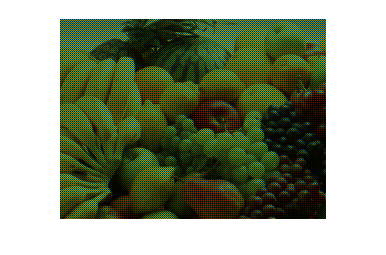
\includegraphics[width=0.47\linewidth] {figures/input}
   \label{fig:input_iters}
 }
 \subfigure[Demosaiced Output (5k Iterations)]{
   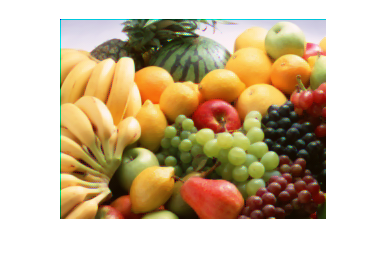
\includegraphics[width=0.47\linewidth] {figures/iters/output_5k}
   \label{fig:output_iters}
 }
 ~
  \subfigure[500 Iterations]{
   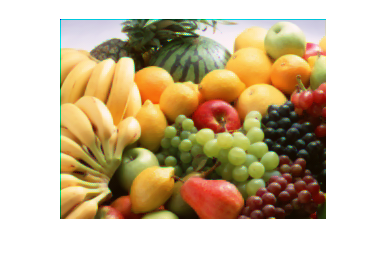
\includegraphics[width=0.30\linewidth] {figures/iters/500}
   \label{fig:500_iters}
 }
 \subfigure[250 Iterations]{
   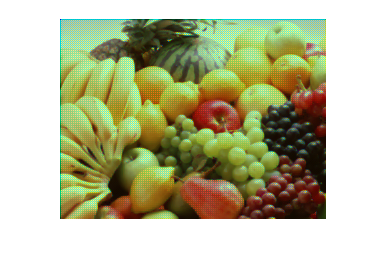
\includegraphics[width=0.30\linewidth] {figures/iters/250}
   \label{fig:250_iters}
 }
 \subfigure[100 Iterations]{
   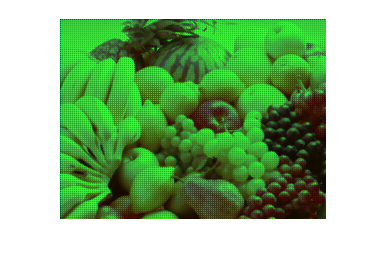
\includegraphics[width=0.30\linewidth] {figures/iters/100}
   \label{fig:100_iters}
 } 
\end{center}
\caption{Demosaiced image using the $\lambda=1000$ and different number of iterations. We observe that when only using 500 iteration we obtain a persuading demosaiced result image.}
\label{fig:varying_iters}
\end{figure}

Next, I experimented with the parameter $\lambda$. I was asking myself what happens when I use a fixed number of iterations and a varying parameter $\lambda$. Results are shown in figure $\ref{fig:varying_lambdas}$. For generating these results, I used 1000 iterations for each demosaiced image. Having a closer look at the produced demosaiced images, we can observe to main findings. First, the lower $\lambda$ gets, the blurrier the result becomes. And and second: Lower values of $\lambda$ affect the results in a way that they are less converged. Both finding actually make sense. The blurriness result for lower $\lambda$ values can be understood when we ask ourself the following question: \emph{on what optimization term is $\lambda$ applied to}? And we see then, that $\lambda$ is multiplied onto the energy term that regularizes the blurriness. Please refer for further insight to the report of the first project. The same reasoning I used there can be applied here. For too small $\lambda$ values we have no convergence anymore. For large enough lambda values there is convergence and also no blur noticeable. Large enough means about $\lambda = 100$.

\begin{figure}[H]
\begin{center}
  \subfigure[$\lambda=1000$]{
   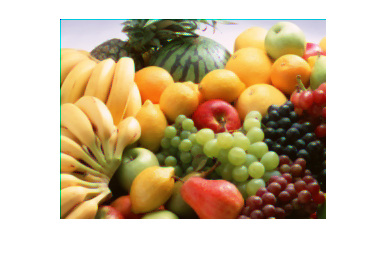
\includegraphics[width=0.30\linewidth] {figures/lambdas/1000}
   \label{fig:500_iters}
 }
 \subfigure[$\lambda=100$]{
   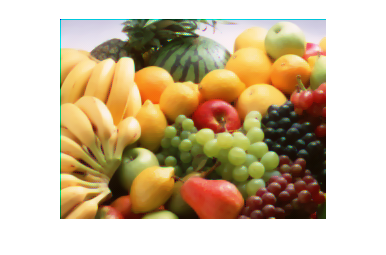
\includegraphics[width=0.30\linewidth] {figures/lambdas/100}
   \label{fig:250_iters}
 }
 \subfigure[$\lambda=10$]{
   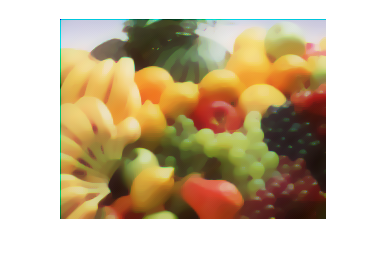
\includegraphics[width=0.30\linewidth] {figures/lambdas/10}
   \label{fig:100_iters}
 }
  ~
  \subfigure[$\lambda=5$]{
   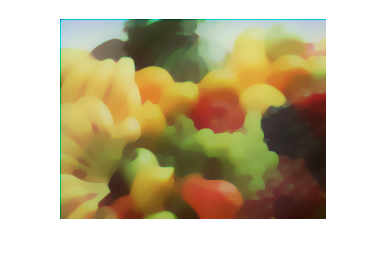
\includegraphics[width=0.30\linewidth] {figures/lambdas/5}
   \label{fig:500_iters}
 }
 \subfigure[$\lambda=2$]{
   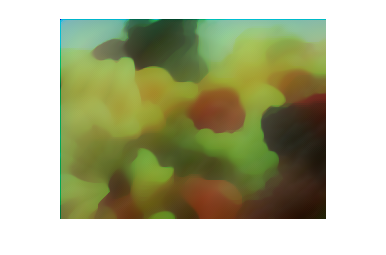
\includegraphics[width=0.30\linewidth] {figures/lambdas/2}
   \label{fig:250_iters}
 }
 \subfigure[$\lambda=1$]{
   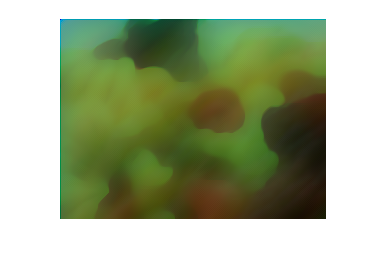
\includegraphics[width=0.30\linewidth] {figures/lambdas/1}
   \label{fig:100_iters}
 }  
\end{center}
\caption{Demosaiced image using 1000 iterations and varying values for $\lambda$. We observe that the smaller $\lambda$ gets, the blurrier the result becomes and also that smaller $\lambda$ affect the convergence of the result in a way that it is less converted (i.e. would require more iterations).}
\label{fig:varying_lambdas}
\end{figure}

The idea how I determined the best $\lambda$ is rather simple: For a fixed number of iterations$\footnote{I used 100 Iterations. I assume that the best determined value for a small number of iterations is also the best $\lambda$ value for a large number of iterations. }$, I run my primal dual solver several times for different $\lambda$ values. For each intermediate result, I computed the SSD between the currently computed demosaiced image and the ground truth image. As we notice this is actually the same approach as I used in the first project. In addition I initially fixed the parameters $\tau$, $\sigma$ and $\theta$ (as described in the implementation section).

The results of the ssd vs lambda plots for the mosaiced fruits iamge are shown in figure $\ref{fig:ssd_vs_lambda}$. 

\begin{figure}[H]
\begin{center}
  \subfigure[SSD vs Lambda Plot]{
   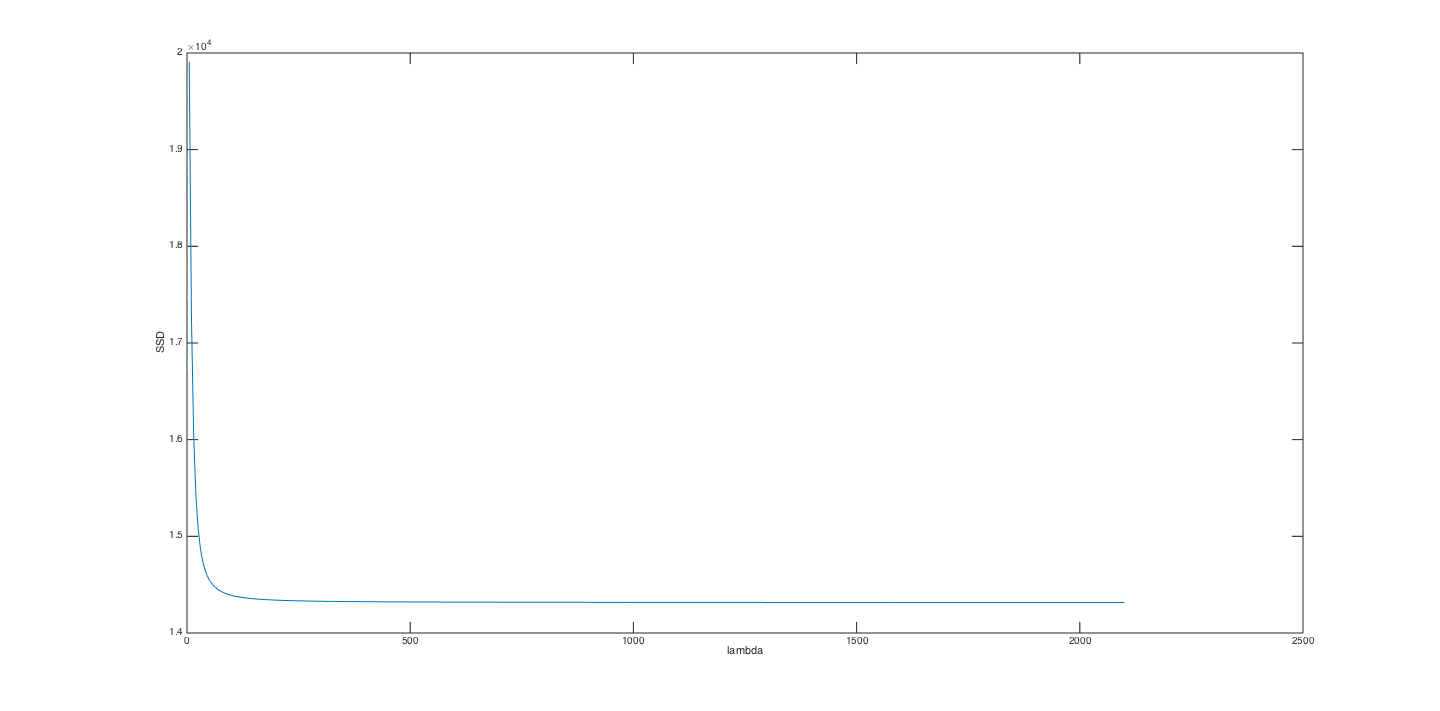
\includegraphics[width=1.0\linewidth] {figures/ssd_vs_lambda}
   \label{fig:500_iters}
 }
\end{center}
\caption{Plotting the SSD vs $\lambda$ for the fruits mosaiced image.}
\label{fig:ssd_vs_lambda}
\end{figure}

Although, the SSD error is already very small for lambda values about 200,  numerically, I determined the value $\lambda = 2105$ as the best $\lambda$ value. The reason for this is that the SSD as a function of lambda is still decreasing for larger values of lambda equal 200 (but indeed very slowly). 

Last, I have also generated a plot for the energy term vs number of iteration. This plot is illustrated in figure $\ref{fig:energy_vs_iterations}$. We observe that after 400 - 500 iterations we are within a error range of zero using the optimal value. In addition I have also plotted the log diff plot of the energy terms shown in figure $\ref{fig:log_diff_energy_vs_iterations}$. This Plot shows the difference between the current energy and the previously computed energy in a log scale. From these plots we can conclude that we usually have to expect to run about 400-500 iterations until we have a good convergence.

\begin{figure}[H]
\begin{center}
  \subfigure[Energy vs Iterations Plot]{
   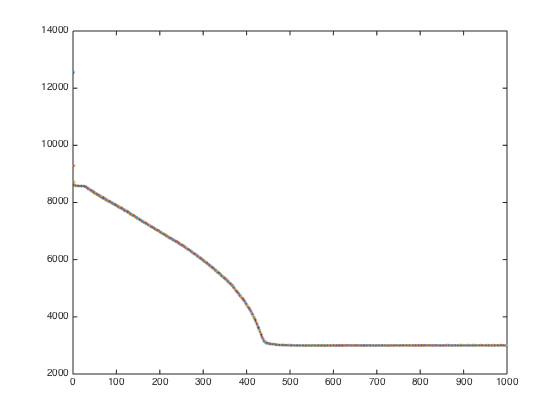
\includegraphics[width=1.0\linewidth] {figures/energy_term}
   \label{fig:500_iters}
 }
\end{center}
\caption{Plotting the Energy vs number of iterations plot for the fruits mosaiced image.}
\label{fig:energy_vs_iterations}
\end{figure}

\begin{figure}[H]
\begin{center}
  \subfigure[Log difference Energy vs Iterations Plot]{
   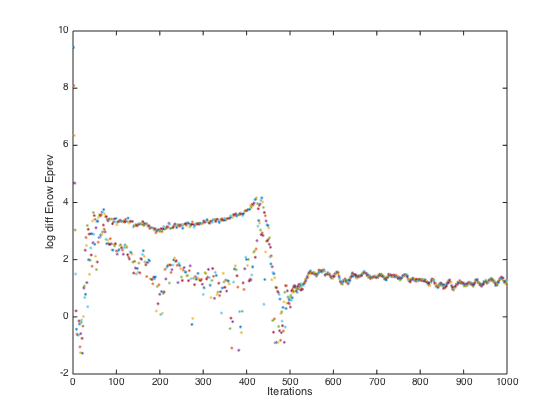
\includegraphics[width=1.0\linewidth] {figures/log_diff_energy_term}
   \label{fig:500_iters}
 }
\end{center}
\caption{Plotting the Energy difference (current energy term minus previous computed Energy) vs number of iterations plot for the fruits mosaiced image of red color channel. Note that I transformed the error into a log space (by applying the log).}
\label{fig:log_diff_energy_vs_iterations}
\end{figure}

Last, a result produced when using all best parameter values and a minimal number of iterations. The result is shown in figure $\ref{fig:best_results}$. When only using 450 iterations and the best lambda value equal 2105 I get a good looking demosaiced result.

\begin{figure}[H]
\begin{center}
  \subfigure[Mosaiced, Demosaiced and intermediate results]{
   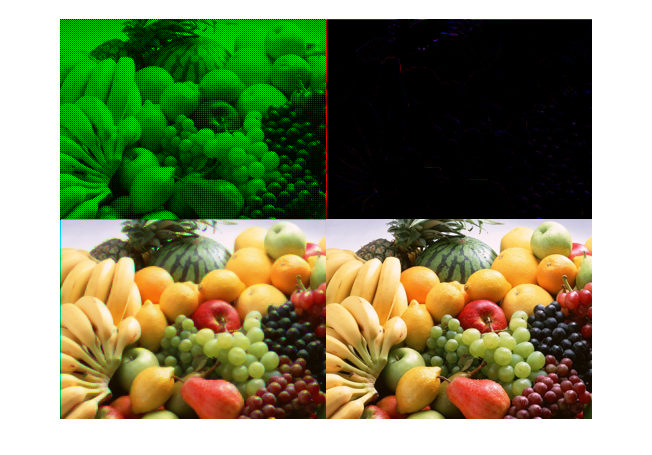
\includegraphics[width=1.0\linewidth] {figures/best}
   \label{fig:500_iters}
 }
\end{center}
\caption{Mosaiced image (left, top), and its demosaiced version (bottom left) using the best lambda value and only 450 iterations. On the right top, the SSD image and on bottom right the ground truth image}
\label{fig:best_results}
\end{figure}


% display 
\section{Conclusion}

In this report we have seen a derivation to solve the demosaicing problem using a primal-dual solver. We also explored the parameter space of that solver and how it converges. Last we compare the prima-dual solver against the gradient descent solver.

The the computational cost of one step in the primal-dual solver is larger than one in the gradient descent method. Reason: Both solvers use inputs of the same dimensionality, however, the primal-dual solver computes several times the gradient of its values (gradient on x, divergence (which is again the gradient) on y). In the gradient descent solver we usually compute once per iteration a gradient. But the primal dual solver requires way fewer iterations than the gradient descent. When using the best lambda values in both solvers, I needed about 400 iterations to get a converged results using my primal dual solver and about 1000 to 2000 iterations when I use my gradient descent method. 

The primal dual solver has way more parameters that have to be specified by the user: actually, there is $\lambda$, $\theta$, $\sigma$, $\tau$ and in the gradient descent solver we only have $\lambda$ and $\alpha$. It is harder to find appropriate parameters for the primal-dual solver. Furthermore, the primal-dual solver is very sensitive to changing parameter setting and may result in diverging results easily when changing lambda. It also takes a lot of time to find good parameter setting for the primal dual solver compared to the gradient descent solver. 

Another point of view is the required mathematical background in oder to develop a particular solver approach. The mathematical basis for formulating a prima-dual solver is way more sophisticated than defining a primal dual solver.

Therefore we conclude: The gradient descent method is simpler to understand, faster but requires a lot of iterations to converges. The primal-dual solver on the other hand is hard to understand, very sensitive to its parameters, computational expensive per iteration, but usually requires fewer iterations.

Lest a little comparison of the results produced by both solvers using their optimal values and parameter settings. The results are shown in figure $\ref{fig:best_comp}$. This comparison directly confirms our conclusion.

\begin{figure}[H]
\begin{center}
  \subfigure[Gradient Descent]{
   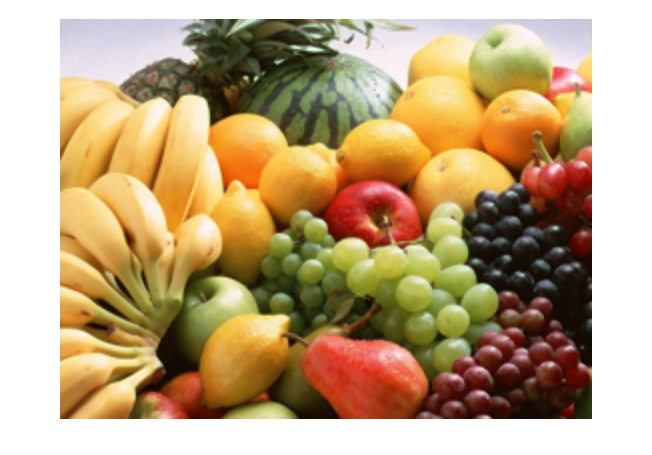
\includegraphics[width=0.8\linewidth] {figures/comp/fruits_l1740i1000Big}
   \label{fig:gd}
 }
  \subfigure[Primal-Dual]{
   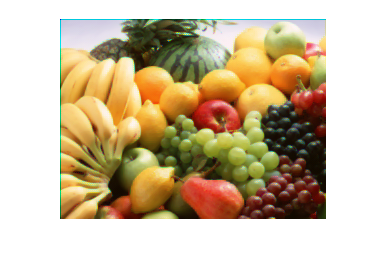
\includegraphics[width=0.95\linewidth] {figures/comp/primal_dual}
   \label{fig:pd}
 }
\end{center}
\caption{Direct companions between the best result produced by the gradient descent solver and the primal-dual solver. I used 400 iterations for the prima-dual, and 1000 for the gradient descent method. The bluish border in the primal dual result can be ignored since this us a result of the zero padding. The same border effect appears when we use a zero padding boundary condition for the gradient solver. I simply have not adapted the code to have a symmetric boundary condition in the primal dual solver.}
\label{fig:best_comp}
\end{figure}

Last, The primal-dual approach also becomes hard to address for operators with unknown norms.

\end{document}











